\documentclass[oribibl]{llncs}
\usepackage{graphicx}
\usepackage{amsmath}
\usepackage{textcomp}       % additional symbols using companion encoding TS1

\title{Collabot}
\subtitle{A Collaborative Robotic Agent for the CiberRato Competition}
\author{Pedro Pontes \and Tiago Varela}
\institute{Faculdade de Engenharia da Universidade do Porto}

%
\begin{document}
\maketitle
\begin{abstract}
This paper discusses the implementation of navigation and target localization strategies for a  collaborative robotic agent, using the Ciber-Rato Simulation Tools. Communication and mapping strategies were also implemented in the discussed agent, however those implementations are further explained in the paper \cite{baboehelder}.
We focused on developing an interesting solution for a maze solver agent and explore the collaboration between robots with similar architectures.
\end{abstract}

\section{Introduction}
Ciber-Rato is a category of the Micro-Rato contest from University of Aveiro.
This category is a competition between small autonomous robots trying to solve mazes. \cite{Lau2002}
In this project, we faced the challenge of developing a collaborative robotic agent architecture using the Simulation Tools created for the Ciber-Rato competition. The agents should be able to solve simple mazes by finding a beacon and returning to their original position, while avoiding obstacles, collisions and dealing with time constraints. Furthermore, in the collaborative competition, the agents are playing in a team of 5 robots, all the robots must meet in the target area and after that return to their original position. The maze is only considered solved when all the mice return to their original position.

At the starting point, the agents have no previous information about the world state, namely the target position, maze's topology and even his or other mice positions. Therefore, a simple reactive robot architecture was not suitable for this problem, so proper communication, mapping, navigation and target localization strategies were be developed in order to maximize the agent's efficiency.

In this paper, first we present the simulation system architecture. Then the agent architecture and design are analysed, mainly focusing in the navigation and target localization strategies, since communication and mapping strategies are further discussed in the paper \cite{baboehelder}. After that, the results of the developed strategies are discussed. Finally, in the last section, are presented the main conclusions and some possible future developments.

\section{Simulation System Architecture}
To develop this project the Ciber-Rato Simulation Tools, 2012 edition, were chosen as a simulation platform. This platform allows the developers to focus only on the development of an efficient agent algorithm, eliminating the problems and challenges associated with real robots construction by providing a simulation environment that models all the hardware components of the robots and a allows the developed algorithms to be tested\cite{Lau2002}. 

The simulation environment is composed by a Simulator, a Simulation Viewer and Virtual Robots. The first is responsible for modelling all the hardware components of the robots, the maze and ensure that all the execution rules are applied. The Simulation Viewer displays the maze, the robots movements and the remaining execution time. The virtual Robots are detailed in the section bellow.

All the specifications presents in this paper are based on the Ciber-Rato 2011 Rules and Technical Specifications \cite{DepartamentodeElectronica2011}, and only a brief specification is present in here, for a more detailed specification please consult the document mentioned above.

\subsection{Virtual Robots}
The virtual robots have circular bodies and are equipped with sensors, actuators and command buttons. Only the robots' sensors and actuators used by the agent that we developed are mentioned in this section.

\subsubsection{Sensors}\hfill \\
For the developed agent the following sensors were used, from the ones available in the simulation environment: 
\begin{itemize}
  \item[\textbf{Obstacle Sensors}]
  4 proximity sensors, 3 oriented to the front of the robot (left, middle and right sides), and one in the rear. Each sensor has a $60^{\circ}$ aperture angle.
  \item[\textbf{Beacon Sensor}]
  Measures the angular position of the beacon with respect to the robot's frontal axis. The measure ranges from $-180$ to $+180$ degrees, with a resolution of 1 degree.
  \item[\textbf{Bumper}]Active when the robot collides.
  \item[\textbf{Ground Sensor}]
  Active when the robot is completely in target area.
  \item[\textbf{Compass}]
  Positioned in the center of the robot and measures its angular position with respect to
the virtual North ($x$ axis).
  \item[\textbf{GPS}]
  Returns the position of the robot in the arena, with resolution 0.1. It is located in the center of the robot.
\end{itemize}

\subsubsection{Actuators}\hfill \\
The actuators components of the robots used in this project are 2 motors and 1 signalling LED. 
\begin{itemize}
  \item[\textbf{Motors}]
Motors have inertia and noise in order to more closely represent real motors, and the translation or rotation movements can be achieved by applying different power values to each motor.
  \item[\textbf{LED}]
The LED is used to signal that the robot has already found the beacon.
\end{itemize}

\subsubsection{Buttons}\hfill \\
Two buttons, named Start and Stop, are provided in each robot and are used by the simulator to start and interrupt the competition.

\subsection{Arena}
The arena is randomly positioned in the world, which means that the starting coordinates of the robot may differ for every attempt to solve the maze, and has a maximum size of $14\times28$ um.
The arena is populated with obstacles, a target area, and a starting grid. For the same maze different starting grids can also be used. The obstacles within the arena can be higher then the beacon, making it invisible for the beacon sensor.

\subsection{Communication}
Communication between robots can be made by sending appropriate commands, through the Simulator. The other agents will be then responsible for reading the messages in the simulator. However the following constraints are be applied:
\begin{itemize}
 \item Per cycle, a robot can send (broadcast) up to 100 bytes;
 \item Per cycle, a robot can read up to 400 bytes;
 \item Robots can only read messages sent from a maximum of 8 units from its current position;
 \item Obstacles do not interfere with communication;
 \item Latency of 1 cycle for sent messages.
 \end{itemize} 

\section{Agent Architecture}
In this project we faced the challenge of creating a team of 5 robotic agents, playing simultaneously, in the environment provided by the Ciber-Rato Simulation Tools.
The Mice have two specific goals: locate the target area and place all the agents inside that area; return all the robots back to their original position.

In order to achieve that goal our agents must be able to fully operate in an unstructured environment by avoiding obstacles and finding the beacon in a simple to moderately complex map. 
However, at the starting point, the agents have no previous information about the world state, namely the target position, maze's topology and even his or other mice positions. Therefore, a simple reactive robot architecture was not suitable for this problem and so proper communication, mapping, navigation and target localization strategies were be developed in order to maximize the agents efficiency.

The developed agent architecture is composed by 6 different modules and is represented in figure \ref{fig:robot-arch}.

\begin{figure}
  \centering
  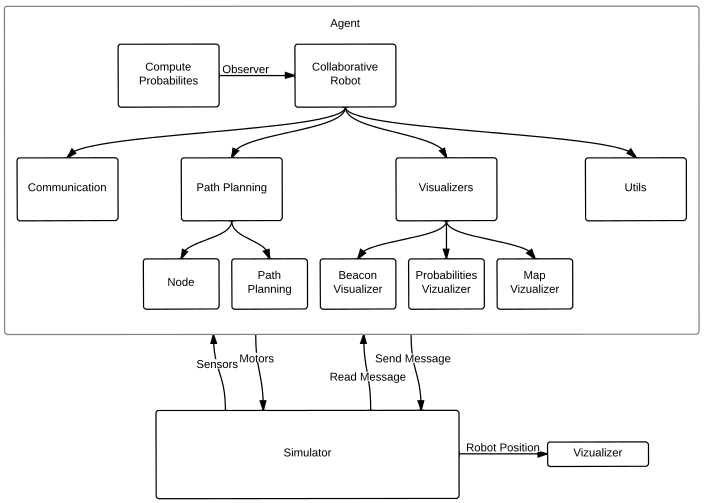
\includegraphics[width=0.9\textwidth]{robot-architecture.png}
  \caption{System architecture.}
  \label{fig:robot-arch}
\end{figure}

Bellow, the description of each module:

\begin{itemize}
  \item[\textbf{Compute Probabilities}]
  lorem ipsum
  \item[\textbf{Communication}]
  lorem ipsum
  \item[\textbf{Path Planning}]
  lorem ipsum
  \item[\textbf{Visualizers}]
  lorem ipsum
  \item[\textbf{Utils}]
  lorem ipsum
\end{itemize}

\subsection{Navigation Strategy}
The navigation strategy followed by our robot can be divided in two fundamental steps: exploring the map before finding and reaching the beacon and returning home after finding it.

\subsubsection{Exploring the Map}\hfill \\

For the first phase of navigation the behavior of our mouse was mostly imported from a previously created solution of a purely reactive mouse described in \cite{Moreira2012}. This solution was inspired by the subsumption layered model that Brooks proposed for mobile robot control system\cite{Brooks_1986}, and can be viewed on figure \ref{fig:layered}.

\begin{figure}
  \centering
  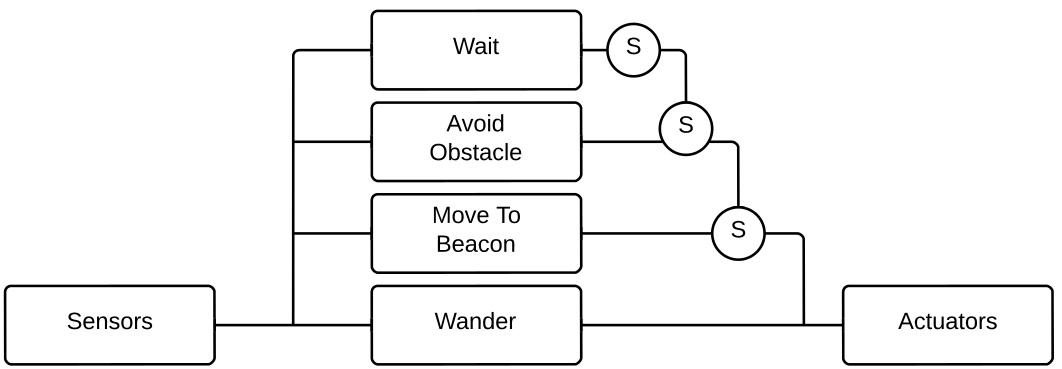
\includegraphics[width=0.8\textwidth]{layer-architecture.png}
  \caption{Layered architecture.}
  \label{fig:layered}
\end{figure}

With this system architecture the top layers are activated when certain conditions are detected by the sensors, overriding the actions of the bottom layers, e.g. if an obstacle is detected the robot will start its obstacle avoidance routine, instead of moving towards the beacon or wandering around. 

Each of these layers will now be described in further detail:

\begin{itemize}
  \item[\textbf{Wait}]
  This layer is used to detect if the robot has reached the beacon location and to stop its motion, also signalling to the Simulator that the robot has finished the first phase of the competition.
  \item[\textbf{Avoid Obstacle}]
  In order to avoid obstacles a wall following algorithm was implemented. The mouse moves always in a clockwise direction and the strategy is held until the beacon is framed within $20^{\circ}$ degrees of amplitude.
  
  One example of a complex obstacle that can be avoided by this algorithm is represented in figure \ref{fig:obstacle1}. At first, the robot is moving forward. When a wall is detected in front of the robot, it turns about $90^{\circ}$ to the right, and keeps moving forward. On every inner corner, $C$, the mechanism is similar to the previously described. On every outer corner, $E$, the robot deviates itself in order to turn and move forward without touching the corner. When the robot is rotating, it verifies if the beacon is visible within a $20^{\circ}$ amplitude, and if that is the case the wall following is aborted and the robot moves in the direction of the beacon.
  
  \item[\textbf{Move to Beacon}]
  This layer detects if the beacon is visible and if it is the robot rotates itself to align with the beacon direction and then moves forward. This rotation value is calculated accordingly to beacon sensor information, e.g. if the beacon direction is opposite to the robot's facing direction then the rotation value is higher than if the beacon direction was only to the left or to the right of the robot.
  When the beacon is not visible the robot finds in it's beacon probability matrix the most
probable location of the beacon, if any, and tries to head in that direction. Details of how this is implemented are available in section \ref{sec:target-loc}.
  
  \item[\textbf{Wander}]
  This layer provides the default action which is for the robot to move around the arena until it finds a wall to follow or sees the beacon.
\end{itemize}
\hfill \\
\begin{figure}
  \centering
  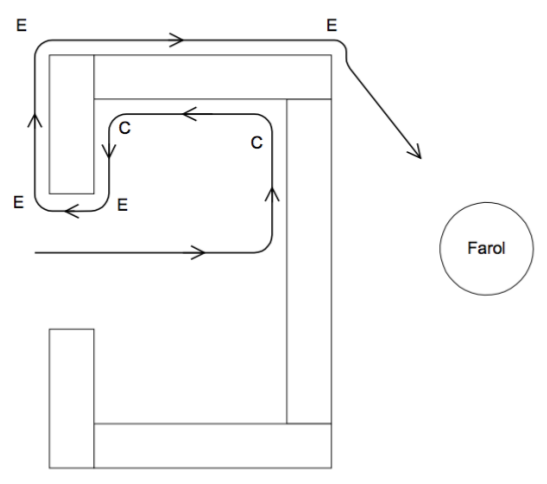
\includegraphics[width=0.6\textwidth]{obstaculo1.png}
  \caption{Example of an obstacle that can be avoided.}
  \label{fig:obstacle1}
\end{figure}

\subsubsection{Return Home}\hfill \\

In order to make the robots return to their original position the robot uses the information gathered until that moment by him and the information collected by the other robots, and calculates the best path using the path planning strategy detailed in the next section of this report. After that, the robot simply iterates through each node of the calculated path, aligns himself with the direction of the child node and then moves forward. This cycle is repeated until the robot reaches its original position.

\subsection{Path Planning}
\label{sec:path-planning}
The path planing problem in the developed solution consists in finding the best possible path between the beacon area and the original position of the robot, considering the information about the world that the robot gathered until that moment. In order to solve this problem Collabot implements an A* algorithm[] in the Path Planning module. The A* algorithm uses a best-first search based on an heuristic to find the path with the lower cost between the initial and goal points in a map.

The Path Planning module is composed by two classes, Node and PathFinder, and it implementation is not coupled to the robotic agent implementation, meaning that this module could be used to solve any problem requiring the shortest path between two points in a two dimensional matrix of doubles. Each cell of the the matrix encapsulates the cost of traveling through that cell, however if the value of a cell is higher than a preset value, the cell is considered to have an obstacle and so is not traversable. Furthermore, all the surrounding cells of a cell are considered as a neighbor, therefore in best possible situation a cell can have 8 neighbors. A cell that is not traversable is not considered as a neighbor of any cell.

To find the best possible path between two points the A* uses an heuristic function to determine the order in which nodes are visited during the search for that path. Equation 1 defines the cost function \textit{f(x)} as the sum of the distance so far traveled, \textit{g(x)}, and the estimated distance to the target, \textit{h(x)}. The estimated distance to the target, represented in equation 2, is computed using the euclidean distance[] between the current point, \textit{p}, and the goal point, \textit{q}, and returns the length of the line segment connecting the two points.

\begin{equation}
f(x) = g(x) + h(x)
\end{equation}

\begin{equation}
h(x) = \sqrt{(p_x - q_x)^2 + (p_y - q_y)^2}
\end{equation}

Finally, in order to ensure that is always possible to travel through the calculated path without touching the walls, the implemented solution also allows the enlargement of the walls of the the maze in the size of the robot radius. To do so, for every node, \textit{N}, of the provided matrix that is not traversable and has not been visited yet, the surroundings nodes, are calculated and the node \textit{N} is marked as visited. If the cost of a surrounding node, \textit{S}, is smaller then the cost of the current node \textit{N}, the cost of \textit{S} is updated to the cost of \textit{N} and \textit{S} is marked as visited.

The path planning module requires a proper world state representation when calculating the shortest path, otherwise the algorithm may calculate paths that are impossible for a robot to cross (i.e. If a cell that contains a obstacle is present in the calculated path). Therefore, to create a more robust test set, two different solutions were explored:
\begin{enumerate}
\item The first was to use the computed probabilities matrix. Originally all the cells of the matrix have the value of 0.5, meaning that the probability of that cell having or not an obstacle is the same. While the robot moves through the arena the values of the matrix are updated. A higher value, means that the probability of having a obstacle in that cell is higher. The algorithm used to update this matrix is further explained in the paper \cite{baboehelder}. Nevertheless, while using this algorithm it is important to ensure that the calculated path always keeps a sufficient distance from the wall, thus it is required to enlarge the walls when using this strategy.

\item The second strategy chosen was to use only the points that were crossed by the robot to calculate the path. With this strategy, the problems related to the sensors noise, or errors in the calculation of the location of the obstacles in the map are avoided, since the robots, only travel through the same tracks they have already crossed. Furthermore, in this strategy, the enlargement of the walls is not required, and the path planning executes faster. However, by not taking all the information available into account, the calculated path may also not be the shortest one.
\end{enumerate}

The results of both strategies are further detailed in the section Results of this paper.

\subsection{Target Localization}
\label{sec:target-loc}
\subsubsection{Storing and visualization}\hfill \\

As mentioned on the Virtual Robots section the agent has a ``Beacon''
sensor that returns the goal's direction, when it is visible. This direction
is measured in 1 degree intervals, the values range from $-$180 to +180 degrees and
are relative to the agent's orientation. The simulator introduces noise to this sensor
using a normal distribution with mean 0 and standard deviation of 2.

To store this information we created a matrix with the same size as the
mapping matrix, a $14\times28$ matrix with each of the axis multiplied by the resolution
used (10), resulting in a $140\times280$ matrix. Using the beacon sensor direction and the
robot's position and orientation we draw a ray on the matrix starting on the agent's
position and aimed at the beacon.

To achieve this we calculate the possible beacon direction and the starting and ending
angle for the ray.
\begin{equation}
BeaconDir = AgentDir + BeaconRelativeDir
\end{equation}
\begin{equation}
StartAngle = BeaconDir - 1
\end{equation}
\begin{equation}
EndAngle = BeaconDir + 1
\end{equation}

After the values are normalized to be in the range of $-\pi$ to $\pi$ we can now
iterate through the matrix and calculate the angle of each
point relative to the agent's position using the $atan2$ function.
The values are normalized because the $atan2$ function also returns values in the range of
$-\pi$ to $\pi$.
\begin{equation}
PntAngle = atan2(AgentY - MatrixPntY, MatrixPntX - AgentX);
\end{equation}

If the $PntAngle$ is in between the $StartAngle$ and the $EndAngle$ then that point in the
matrix is incremented by 1.

The visualizer represents this values using different color ranges:
\begin{itemize}
  \item[\textbf{Yellow}] For values below 8
  \item[\textbf{Orange}] For values between 8 and 12
  \item[\textbf{Red}] For values between 12 and 100
  \item[\textbf{Black}]For values larger than 100
\end{itemize}

\begin{figure}
  \centering
  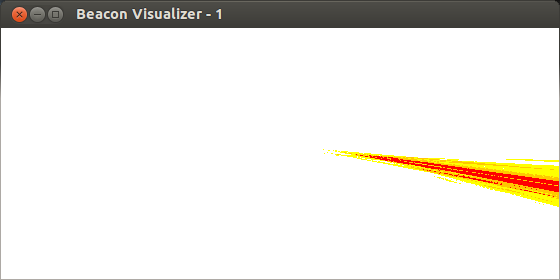
\includegraphics[width=0.8\textwidth]{beacon-1.png}
  \caption{Beacon visualizer with beacon on the right and robot on the left.}
  \label{fig:beacon1}
\end{figure}

Figure \ref{fig:beacon1} represents the beacon visualizer after the first sightings
of the objective in a map where the beacon is on the right and the agent starts
on the left.

\subsubsection{Using the information}\hfill \\

When the agent is searching for the beacon and the sensor is available it always
uses that information to align itself with the target, because that information is the
most recent and the most accurate one.

However, if the sensor is not available, because the path is obstructed by a wall,
and the agent has some information stored in the beacon probability matrix, he searches for
the highest value on the matrix and uses the position where that value is to align
itself to that direction.

\section{Results}

\subsection{Navigation Strategy}
As stated in the section 3.1 of this report, the navigation strategy followed by our agent in its first phase of map exploration is mostly reactive and imported from the solution described in \cite{Moreira2012}. This solution, has some well known problems of reactive solutions, namely in solving some types of corners or cycles. Due to time constrains and the specific goal of this project, in our solution we didn't approach such problems. For a more detailed info in this specific solution \cite{Moreira2012} should be consulted.

In order to store the robot movements and location to update the map, we decided to use the same approach of YAM \cite{Ribeiro2002}, since the solution developed by its authors was already validated by winning a the ciber mouse competition in 2002. 
To a cycle n, if X[n] is the horizontal axis coordinate, Y[n] the vertical one, D[n] the power applied to the right motor, E[n] the power applied to the left one and $\theta[n]$ the orientation given by the compass, so:
\begin{equation}
Lin[n] = (D[n] + E[n]) / 2.0
\end{equation}
\begin{equation}
X[n+1] = X[n] + cos(θ[n]).Lin[n]
\end{equation}
\begin{equation}
Y[n+1] = X[n] + sen(θ[n]).Lin[n]
\end{equation}

Despite the good results obtained when using this approach to map the walls off the map, when using this solution to follow a specific path (i.e. return home), the precision of the method has proven to be low, and so in order to further evolve our work, we decided to use the GPS sensor (without noise), to map the robot position in  those situations.

\subsection{Path Planning}
To assess the performance of the path planing strategy a lot of tests were done. Bellow, a demonstrative example of a complex map is analysed. 

The path returned by the path planning algorithm is represented in green, the areas that we have no information about are represented in white. The obstacles are represented in a gradient from white to red. A cell is more red if the probability of having a wall is higher. The same reasoning is applied to represent the areas without obstacles in a gradient from white to black.

In figure \ref{fig:map} the original map is represented. Figures \ref{fig:pathProb} and  \ref{fig:pathProbEnlarge} represent the calculated path by the second method described in section \ref{sec:path-planning} of this paper, without and with wall growing respectively. Figure \ref{fig:pathAStar} represents the same problem resolved by using the second method described in \ref{sec:path-planning}.

\begin{figure}[ht]
\begin{minipage}[b]{0.45\linewidth}
\centering
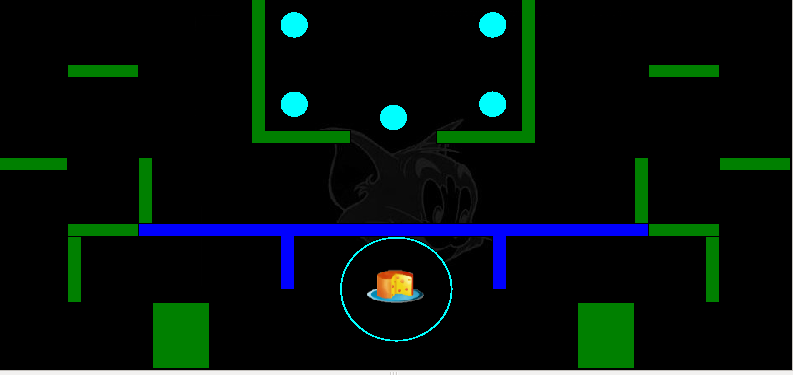
\includegraphics[width=\textwidth]{map.png}
\caption{CiberRTSS08 Stage 2 Map.}
\label{fig:map}
\end{minipage}
\hspace{0.5cm}
\begin{minipage}[b]{0.45\linewidth}
\centering
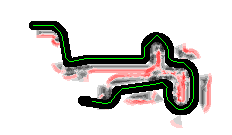
\includegraphics[width=\textwidth]{pathAStar.png}
\caption{Calculated Path method 2.}
\label{fig:pathAStar}
\end{minipage}
\end{figure}

\begin{figure}[ht]
\begin{minipage}[b]{0.45\linewidth}
\centering
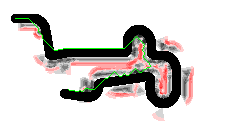
\includegraphics[width=\textwidth]{pathProb.png}
\caption{Calculated Path method 1.}
\label{fig:pathProb}
\end{minipage}
\hspace{0.5cm}
\begin{minipage}[b]{0.45\linewidth}
\centering
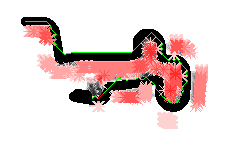
\includegraphics[width=\textwidth]{pathProbEnlarge.png}
\caption{Calculated Path method 1, with wall growing.}
\label{fig:pathProbEnlarge}
\end{minipage}
\end{figure}

As it is possible to observe in the figures, the results showed that when using the calculated probabilities matrix it is essential to grow the walls before calculating the returning path, otherwise the path will be impossible for the robot to cross. This can be explained by two motives: First, the noise of the sensors can lead to bad mapping of the walls, making cells be marked with a low probability when there is actually a wall on them. Secondly, even if the walls are properly mapped, the returned path is often to close to corners and walls, producing a lot of collisions when being followed. Both problems are illustrated in figure \ref{fig:pathProb}.

Finally, when comparing the results obtained by both methods it is clear that, for our solution, method 2 has proven to produce better results. By not having to deal with problems related to bad mapping of obstacles and even the size of the walls, the calculated path is always possible to cross since it has already been by the robot before. Furthermore, the wall growing method developed, produces a lot of noise, making the calculated path, more difficult to follow, since a lot of direction changes have to be done.


\subsection{Target Localization}
The target localization used in this agent was inspired by the method used on the
YAM robotic agent.\cite{Ribeiro2002}

This method creates \textit{beacon heat maps} where it is easy to visualize an approximate
area for the location of the beacon. This can seen on figure \ref{fig:beaconXX}.

However, one of the disadvantages of the way this method was implemented is that when the agent
is moving towards the beacon it creates a large area with high probability past the beacon.
In figure \ref{fig:beacon1} cones with high probability are represented and the beacon is only in a small area of that cone.


\section{Conclusion e Future Work}
era bonito usar mais a colaboracao.
Filtros de kalman para o GPS

\bibliography{report}
\bibliographystyle{splncs}
\end{document}